%% Refer elsdoc for options available for "Document Class"
\documentclass[3p]{elsarticle}

%% \usepackage{lineno}
\usepackage{lineno,hyperref}
% if you have landscape tables
\usepackage[figuresright]{rotating}

%% Custom Packages
%%\usepackage{fixltx2e} %% For SubScript
\usepackage{float} %% For image placement
\usepackage{multirow} %% For Multi-Row functionality in tables

%% Put line numbers for every line.
\modulolinenumbers[1] 

%% Enter Journal Name here
\journal{Materials and Design}
%%%%%%%%%%%%%%%%%%%%%%%%%%%%%%%%%%%%%%%%%%%%%%%%%%%%%%%%%%%%%%%%%%%%%%%%%%

%% The amssymb package provides various useful mathematical symbols
\usepackage{amssymb} 
%% The amsmath package provides various useful mathematical formulae
\usepackage{amsmath}
%% The amsthm package provides extended theorem environments
%% \usepackage{amsthm}

%%%%%%%%%%%%%%%%%%%%%%%
%% Reference Styling %%
%%%%%%%%%%%%%%%%%%%%%%%

%% natbib.sty is loaded by default. However, natbib options can be
%% provided with \biboptions{...} command. Following options are
%% valid:

%%   round  -  round parentheses are used (default)
%%   square -  square brackets are used   [option]
%%   curly  -  curly braces are used      {option}
%%   angle  -  angle brackets are used    <option>
%%   semicolon  -  multiple citations separated by semi-colon
%%   colon  - same as semicolon, an earlier confusion
%%   comma  -  separated by comma
%%   numbers-  selects numerical citations
%%   super  -  numerical citations as superscripts
%%   sort   -  sorts multiple citations according to order in ref. list
%%   sort&compress   -  like sort, but also compresses numerical citations
%%   compress - compresses without sorting
%%
%% Example : \biboptions{comma,round}

\biboptions{square,comma,sort&compress}

%%%%%%%%%%%%%%%%%%%%%%%%%%%%%%%%%%%%%%%%%%%%%%%%%%%%%%%%%%%%%%%%%%%%%%%%%%
                   %% Declarations for front matter
\begin{document}
                   %% Declarations of Commands
\newcommand{\degree}{\ensuremath{^{\circ}}}  %% Command for degree

\begin{frontmatter}

\title{Friction welding of Ti-6Al-4V tube to AA6061 tube-plate using an external tool}

%%%%%%%%%%%%%%%%%%%%%%%%%%%%%%%%%%%%%%%%%%%%%%%%%%%%%%%%%%%%%%%%%%%%%%%%%%
                      %% Author Declaration
\author[META]{Sharan. C}
\ead{Sharanc25@gmail.com}
\author[META]{Maxwell Rejil. C}
\ead{maxwellrejilc@gmail.com}
\author[META]{Sachin More}
%\ead{soorajramana89@gmail.com}
\author[META]{Muthukumaran. S\corref{cor1}}
\ead{smuthu@nitt.edu}
%\ead[url]{http://www.nitt.edu/home/academics/departments/meta/faculty/asstprof/smuthu}

\cortext[cor1]{Corresponding Author}

\address[META]{Department of Metallurgical and Materials Engineering, National Institute of Technology, Tiruchirappalli-620015, India}
%%%%%%%%%%%%%%%%%%%%%%%%%%%%%%%%%%%%%%%%%%%%%%%%%%%%%%%%%%%%%%%%%%%%%%%%%%
         
\begin{abstract}
Using a new solid state welding process---Friction welding of tube to tube plate using an external tool (FWTPET), Ti-6Al-4V tube and AA6061-T6 tube plate were welded together. The welding was carried out at 4 different tool rotational speeds (550, 700, 900 and 1100) with two different tube profiles (Holes and Petals). The effect of tube profile on joint strength of the welded samples was measured using an in-house developed test procedure named ``Plunge Shear Test''. Highest weld strength of 192.03 MPa was observed in petals profile welded at 1100 rpm and lowest weld strength of 95.76 MPa was observed for holes profile welded at 550 rpm. Macro and Micro structural studies were done on the welded samples. SEM Fractography studies were carried out on the fractured surfaces after Plunge Shear Test. XRD analysis was done to identify the formation of intermetallics at the joint interface.
\end{abstract}

\begin{keyword}
Ti-6Al-4V \sep AA6061 \sep Friction welding of tube to tube plate \sep Plunge Shear Test \sep Titanium Aluminide \sep  Solid State Welding
\end{keyword}

\end{frontmatter}

%%%%%%%%%%%%%%%%%%%%%%%%%%%%%%%%%%%%%%%%%%%%%%%%%%%%%%%%%%%%%%%%%%%%%%%%%%
							 %%Line Numbers
%% Start line numbering with
%% \begin{linenumbers}, end it with \end{linenumbers}. Or switch it on
%% for the whole article with \linenumbers after \end{frontmatter}.

\linenumbers
%%%%%%%%%%%%%%%%%%%%%%%%%%%%%%%%%%%%%%%%%%%%%%%%%%%%%%%%%%%%%%%%%%%%%%%%%%
							  %%Sections
								
\section{Introduction}
\label{sec:Introduction}
Friction welding of tube to tube plate using an external tool (FWTPET) is a new solid state welding process, invented by one of the present authors, S. Muthukumaran in the year 2006 and patented in the year 2008 (Patent Number - 21744). FWTPET process uses a non-consumable external tool similar to FSW processes, consisting a shoulder and a pin.  In FWTPET, the rotating tool is lowered on to the plate and tube assembly at a constant plunge rate. When the tool touches the plate surface, it produces frictional heat. Unlike FSW process, in FWTPET, the tool pin acts as an anvil and does not cause any stirring action.   This frictional heat along with the axial and rotational forces plasticizes the material and forces the material to flow towards the center of the tube through the flash trap. The tool pin acts as an anvil which drives the material away from the center. These opposing forces, force the plasticized materials to fill the flash trap. The parameters that affect the joint strength of a FWTPET welded joints are : tool rotational speed, tube profile, tool shoulder and pin dimension, heat input etc. The effect on joint strength on different tube profiles, such as holes, zig-zag holes, vertical and horizontal slots were already studied by Senthil Kumaran et al. Their study concluded that holes profile showed the highest joint strength \cite{SenthilKumaran2013}. In our present study, AA6061 tube plate and Ti-6Al-4V tube were welded together using holes profile and a newly designed petals profile. The effect of holes and petals profiles on joint strength was studied.
\par
Highest performance, concurrent weight and cost reduction has become more and more important in aviation industry. There are different approaches to meet these demands. It is well known, for example, that welding of skin-stringer joints is progressively replacing riveted fuselage structures. Another very effective possibility is the implementation of hybrid structures; components made of different materials can be tailored for local needs. There is a rising need for a welding method to join dissimilar materials, such as Titanium (Ti) and Aluminium (Al). However, joining of low melting Al alloys with high temperature Ti alloys is difficult due to the formation of excessive intermetallic compounds at interface by conventional fusion welding method \cite{MadhusudhanReddy2009}. Fusion welding of Al and Ti require the formation of two separate weld pools during welding. This requires precision machined Aluminium–titanium blanks.


%%%%%%%%%%%%%%%%%%%%%%%%%%%%%%%%%%%%%%%%%% Nomenclature %%%%%%%%%%%%%%%%%%%%%%%%%%%%%%%%%%%%%%


\begin{table*}[!t]

\end{table*}

%%%%%%%%%%%%%%%%%%%%%%%%%%%%%%%%%%%%%%%%%%Experimental Details%%%%%%%%%%%%%%%%%%%%%%%%%%%%%%%%%%%%%%

\section{Experimental Details} 
\label{sec:Experimental Details}
\subsection{Materials}
\label{subsec:Materials}
The base materials used for FWTPET process were AA6061-T651 plates and Titanium Grade V (Ti-6Al-4V) tubes. The external tool used for welding was made of Tungsten alloy having 29 mm shoulder diameter and 12.5 mm pin diameter. The chemical composition of AA6061 plate, Ti-6Al-4V tube and Tungsten Alloy Tool is given in Table~\ref{table:base-material-composition}.
\par 
AA6061 plates of 6 mm thickness were cut into 50 x 50 mm squares. A hole of 19 mm diameter was drilled at the center of the plate. Ti-6Al-4V tube of 19 mm outer diameter and 14 mm inner diameter with two tube profiles, holes and petals were used for welding. The details about the tube profile are given below.
\begin{description}
\item [Holes Profile] \hfill \\ 
Holes of 2 mm diameter were drilled at equal intervals along the circumference of the Ti-6Al-4V tubes of height 20 mm. The holes were made at a depth of 5 mm from top of the tube.
\item [Petals Profile] \hfill \\
Slots of 10 mm depth and 2 mm width were made at equal intervals along the circumference of the Ti-6Al-4V tubes of height 30 mm. The slots were then formed into petals using a suitable tool.
\end{description}

\begingroup
\renewcommand*{\arraystretch}{1.5}
\begin{table*}[!htbp]
\caption{Chemical Composition AA6061 Plate, Ti-6Al-4V Tube and Tungsten Alloy Tool (\%wt.)}
\label{table:base-material-composition} % is used to refer this table in the text
\centering
\resizebox{\textwidth}{!}{%
\begin{tabular}{cccccccccccccccccc}
\hline
Alloys & Fe & Cu & Cr & Mn & Zn & C & O & N & H & Co & Ni & Mg & Si & V & W & Al & Ti \\ \hline
AA6061 & 0.497 & 0.164 & 0.148 & 0.045 & 0.004 & - & - & - & - & - & - & 0.70 & 0.43 & - & - & bal. & 0.049 \\
Ti-6Al-4V & 0.03 & - & - & - & - & 0.08 & 0.2 & 0.05 & 0.148 & - & - & - & - & 4.12 & - & 6.04 & bal. \\
Tool & 3.4 & - & - & - & - & - & 0.007 & - & - & 0.2 & 5.3 & - & - & - & 90.5 & - & - \\ \hline
\end{tabular}
}
\end{table*}
\endgroup


\subsection{FWTPET}
\label{subsec:FWTPET}
FWTPET process was carried out in a 4-Axis Friction Stir Welding machine (\ref{fig:fsw-machine}). Before welding, the tube and plate faying surfaces were cleaned with Acetone to remove dirt and grease. The tube and plate were fitted to a specially designed fixture as shown in \ref{fig:backing-block}. The welding parameters used for welding are given in Table \ref{table:process-parameters}. 

\begin{table*}[!htbp]
\caption{FWTPET Process Parameters}
\label{table:process-parameters} % is used to refer this table in the text
\centering
\begin{tabular}{|c|c|}
\hline 
Plunge Depth & 2 mm from plate surface \\ 
\hline 
Plunge Rate & 6 mm/min \\ 
\hline 
Tube Projection & 2.5 mm \\ 
\hline 
Tool Rotational Speed & 550, 700, 900, 1100 RPM \\ 
\hline 
\end{tabular} 
\end{table*}

The 2.5 mm projection helps in pre-heating the tool inorder to achieve better metal flow. It takes 45 seconds to complete one weld for both the holes and tube profile. A total of four welds were made for each tool rotational speed for consistency.

\subsection{Plunge Shear Test}
\label{subsec:Plunge Shear Test}
The weld strength of FWTPET welds are measured using an in-house developed testing procedure called ``Plunge Shear Test''. The strength of a weld can be measured only if the welded specimen fails at the weld interface. PST is a destructive testing method, designed in such a way that the welded specimens fail exactly at the joint interface during testing. PST is carried out on a conventional UTM with the use of an external plunger. PST requires, a specially machined half-solid-half-hollow tube for welding. After welding, the sample is placed in a specially designed fixture and fixed to a UTM. The plunger is used to apply a compressive load on the solid part of the tube at a constant cross-head speed until the joint breaks.  
\par
For our current work, the cross-head speed of the UTM was kept as 3 mm/min. For holes profile, a rod of 19 mm diameter and 30 mm length was taken and a hole of 14 mm diameter was drilled to a depth of 20 mm as shown in Fig. For petals profile, a rod of 19 mm diameter and 35 mm length was taken and a hole of 14 mm diameter was drilled to a depth of 20 mm as shown in Fig. 

\subsection{Characterization}
\label{subsec:Characterization}
The welded samples were sectioned at the weld joint for metallographic studies. Studies were made using a standard stereoscope and optical microscope. SEM and EDS analysis were performed to quantify the elemental weight percentage at the joint interface. The observations were carried out in a 200kV field effect scanning electron microscope (SEM-JEOL JSM 5410LV microscopy) coupled with EDS. EDS line scan was also carried out along the weld interface. XRD analysis was done at the weld interface of Al-Ti dissimilar welds to find out the formation of intermetallics at the weld interface. For XRD, scan speed was 10\degree /min and step width of 0.02\degree was used. In order to reveal the microstructures, a common etchant to etch both AA6061 and Ti-6Al-4V was developed. The etchant consists of equal parts of Ethanol, HCl, HNO$_{3}$ and few drops of HF. The etching time varied between 25 to 40 seconds based on the heat input on the welded samples.

%%%%%%%%%%%%%%%%%%%%%%%%%%%%%%%%%%%%%%%%%%Results and Discussion%%%%%%%%%%%%%%%%%%%%%%%%%%%%%%%%%%%%%%
\section{Results and Discussion}
\label{sec:Results and Discussion}

\subsection{Characterization}
\label{subsec:results-characterization}
The microstructure of AA6061-T651 base metal is shown in Fig. 6. Optical micrographs of the base AA6061-T6 revealed the presence of Mg$_{2}$Si precipitates which strengthens the Al
alloy [4]. After welding, AA6061-T6 showed fine grain structure at the weld interface with dissolution of Mg$_{2}$Si. In case of Ti-6Al-4V, the microstructure at the interface (Fig. 10) shows fine grain structure with equiaxed α phase with inter-granular retained β phase. When we move away from the interface, the
microstructure resembles that of the base metal microstructure for both AA6061-T651 and Ti-6Al-4V.After welding, AA6061-T651 showed fine grain structure at the weld interface with dissolution of Mg$_{2}$Si. Ti-6Al-4V region did not show any microstructural changes. the microstructure at the interface (Fig. 10) shows fine grain structure with equiaxed α phase with inter-granular retained β phase. When we move away from the interface, the microstructure resembles that of the base metal microstructure for both AA6061-T651 and Ti-6Al-4V.

\subsection{Heat Generated during FWTPET}
\label{subsec:Heat Generated during FWTPET}
The heat input rate for FWTPET is given in equation \ref{eq:heat-input}.
\begin{gather} 
\dot{Q} =  \frac{2\pi}{3} \times  \omega \times \tau_{friction} \times (R^{3}_{o} - R^{3}_{i}) \\
Q_{T} = \dot{Q} \times t \label{eq:total-heat-input} \\
\tau_{friction} = \mu \times P \label{eq:Contact-shear-stress}
\end{gather}
where : \\
$\dot{Q}$ is the Heat Generation Rate \\
$Q_{T}$ is the Total Heat Generated \\
$\omega$ is the angular momentum of the tool \\
$\tau_{friction}$ is the contact shear stress \\
$R_{o}$ is the outer radius \\
$R_{i}$ is the inner radius \\
$t$ is the welding time \\
$\mu$ is the co-efficient of friction and\\
$P$ is the normal force during welding.

For our current work, $\mu$ was taken as 0.35 for all the welds. Table \ref{table:total-heat-generated} gives heat generated during FWTPET. 

\begin{table*}[h]
\centering
\caption{Total Heat Generated for Holes Profile during FWTPET }
\label{table:total-heat-generated}
\resizebox{\textwidth}{!}{%
\begin{tabular}{|c|c|c|c|c|c|c|c|c|c|}
\hline
\multirow{2}{*}{RPM} & \multicolumn{2}{c|}{\begin{tabular}[c]{@{}c@{}}Maximum Load\\  (kN)\end{tabular}} & \multicolumn{2}{c|}{\begin{tabular}[c]{@{}c@{}}Contact Shear Stress \\ (N/mm2)\end{tabular}} & \multicolumn{2}{c|}{\begin{tabular}[c]{@{}c@{}}Heat Generation Rate \\ (kJ/s)\end{tabular}} & \multicolumn{2}{c|}{\begin{tabular}[c]{@{}c@{}}Heat Generated\\  (kJ)\end{tabular}} & \multirow{2}{*}{\begin{tabular}[c]{@{}c@{}}Total Heat Generated \\ (kJ)\end{tabular}} \\ \cline{2-9}
 & Tube & Plate & Tube & Plate & Tube & Plate & Tube & Plate &  \\ \hline
\multicolumn{10}{|c|}{Holes Profile} \\ \hline
550 & 18.95 & 7.85 & 43.9 & 4.65 & 2.72 & 1.517 & 68.00 & 30.33 & 98.33 \\ \hline
700 & 18.95 & 7.85 & 43.9 & 4.65 & 3.46 & 1.930 & 86.55 & 38.60 & 125.15 \\ \hline
900 & 18.95 & 7.85 & 43.9 & 4.65 & 4.45 & 2.482 & 111.28 & 49.63 & 160.91 \\ \hline
1100 & 18.95 & 7.85 & 43.9 & 4.65 & 5.44 & 3.033 & 136.01 & 60.66 & 196.67 \\ \hline
\multicolumn{10}{|c|}{Petals Profile} \\ \hline
550 & 20 & 7.85 & 23.76 & 6.20 & 4.61 & 2.02 & 115.23 & 40.44 & 155.67 \\ \hline
700 & 20 & 7.85 & 23.76 & 6.20 & 5.87 & 2.57 & 146.66 & 51.47 & 198.13 \\ \hline
900 & 20 & 7.85 & 23.76 & 6.20 & 7.54 & 3.31 & 188.56 & 66.18 & 254.74 \\ \hline
1100 & 20 & 7.85 & 23.76 & 6.20 & 9.22 & 4.04 & 230.46 & 80.88 & 311.35 \\ \hline
\end{tabular}
}
\end{table*}

\subsection{Weld Strength}
\label{subsec:Weld Strength}
 The fracture load of the weld joint when divided by the area of the weld gives the weld strength \ref{eq:weld-strength}. PST was designed so that the welded specimens fail exactly at the joint interface. After PST, SEM images of the fractured surfaces were taken. Fractography images show river-flow pattern, which indicates shear failure.

\begin{gather} 
Weld\:Strength = \frac{\sigma}{A} \label{eq:weld-strength} \\
Weld\:Area = \pi \times d \times h \label{eq:weld-area}
\end{gather}
where :\\
~$\sigma$ is the fracture load and \\
~$A$ is the weld area. \\
~$d$ is the external diameter of the Ti-6Al-4V tube and \\
~$h$ is the height of weld.

The weld area of FWTPET joints is equal to the lateral surface area of the cylindrical tube, where the height is equal to the thickness of the plate. In our case, due to the 2 mm plunge depth on the plate surface, the height of the weld was taken as 4 mm. The weld area calculated was circa 238.76 mm$^{2}$. For all speeds, the petals profile showed higher joint strength compared to the holes profile. Values for different tube profiles are given in Fig. \ref{fig:weld-strength}. From the table, it is clear that tube with petals is having high shear strength compared to other to profiles.



\subsection{X-Ray Diffraction Analysis}
\label{subsec:XRD-Results}

\subsubsection{Williamson Hall}
\label{subsec:Williamson-Hall}




\subsubsection{Dislocation Density}
\label{subsec:Dislocation-Denstiy}
\begin{align} 
\rho  &= \frac{[2Ad^{2} \times \Delta d \times D^{2}]-[0.9^{2} \times 2A \times d^{2}]}{\pi \times b^{2} \times \bar{c} \times D^{2}} \label{eq:Dislocation-Denstiy} \\
\bar{c} &= a[1-e^{\frac{-A_{i}}{b}}] + C \times A_{i} + d \label{eq:C-bar} \\
A_{i} &= \frac{2 \times C_{44}}{C_{11} - C_{12}} \label{eq:ai}
\end{align}
where :\\
~$\rho$ is the Dislocation Density \\
~$A$ is Constant (3.3) \\
~$d$ is the d-spacing \\
~$\Delta d$ is the FWHM (in radians)
~$\bar{c}$ is the contrast factor
~$\bar{c}$ is the contrast factor

The dislocation density at the weld interface was studied using modified Williamson-hall equation.
XRD plot at the weld interface for welds made with Tube with petals is shown in Fig\ref{fig:xrd-plot}. From the XRD plot, the presence of TiAl$_{3}$ intermetallic formation was observed. Formation of intermetallic compounds is detrimental to joint strength. Titanium aluminide has three major intermetallic compounds: γ TiAl, α Ti$_{3}$Al and TiAl$_{3}$. Although these intermetallics have very good mechanical and thermal properties, they have very low ductility [6]. Therefore, the presence of Titanium aluminides at the interface might decrease the joint strength.



\subsection{Fractography}
\label{subsec:Fractography}
The SEM image (Fig. 15) shows fracture surface of Titanium tube for petal profile after the PST. From the image, we can clearly see some areas on the fracture surface where the aluminum alloy is still bonded to Titanium. SEM images of the fracture surface on the Aluminum plate shows cleavage facets, which is an indication shear fracture [7],[8]. Some Titanium particles embedded in the Aluminium matrix are also visible in
the SEM images (Fig. 16 b).

\section{Conclusion}
\label{sec:Conclusion}
\begin{enumerate}[1.]
\item FWTPET method has been established to join 6mm thick Aluminum (AA6061-T651) tube plate to Titanium (Ti-6Al-4V) tubes of 2.5mm wall thickness.
\item Three different tube profiles-hole, slot and petals, were used to study the feasibility of joining dissimilar materials (Al-Ti) using FWTPET and petal profile was found to have good strength.
\item Shear strength of the joint reached 60\% of AA6061–T651 base material strength.
\item XRD analysis showed formation of TiAl$_{3}$ at the interface. Intermetallic compounds at the interface were less when compared to traditional fusion welding processes which is due to the reduction in heat generation during the welding process.
\end{enumerate}


%%%%%%%%%%%%%%%%%%%%%%%%%%%%%%%% Hides all Images %%%%%%%%%%%%%%%%%%%%%%%%%%%%%%%%%

\iffalse

\begin{figure*}[H]
\centering
\includegraphics[width=\textwidth,height=\textheight,keepaspectratio]{images/"xrd".png}
\caption{XRD - Plot}
\label{fig:xrd-plot}
\end{figure*}


\begin{figure}[!htbp]
\centering
\includegraphics[width=\textwidth,height=\textheight,keepaspectratio]{images/"welding-set-up".png}
\caption{XRD - Plot}
\label{fig:xrd-plot}
\end{figure}


\begin{figure}[H]
\centering
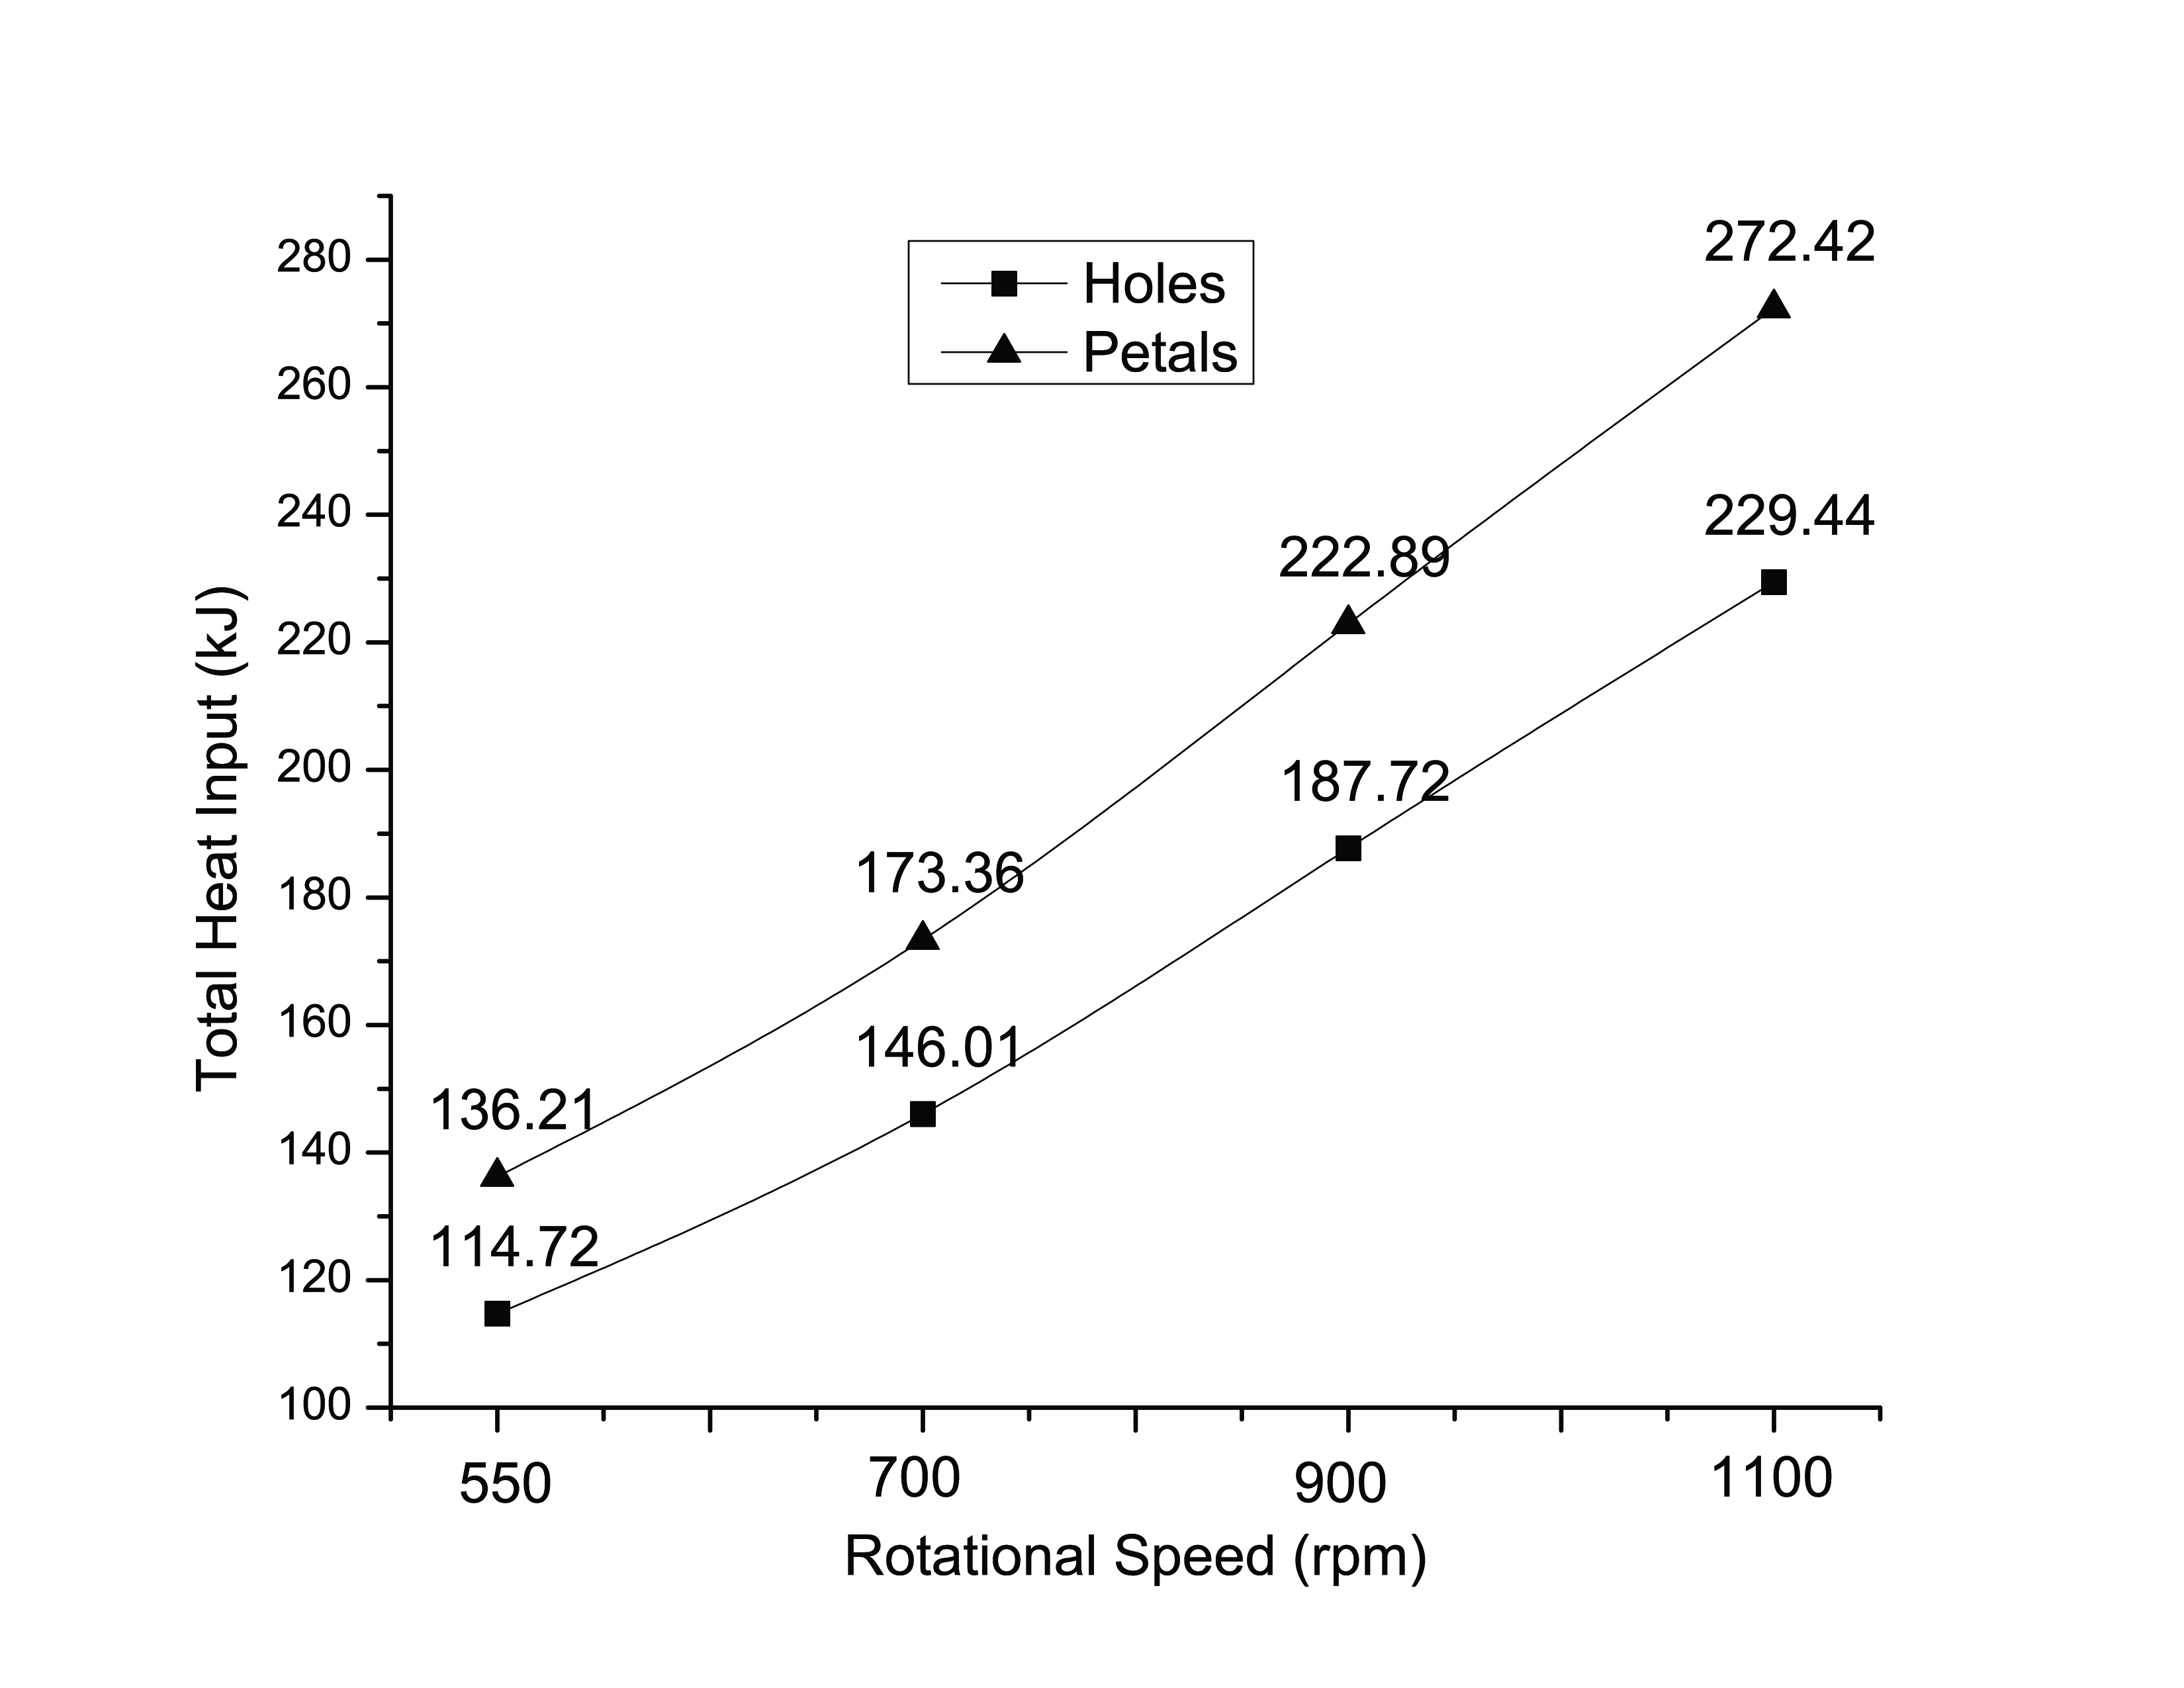
\includegraphics[width=\textwidth,keepaspectratio]{images/Total HI.jpg}
\caption{Total Heat Input during FWTPET}
\label{fig:total-heat-input}
\end{figure}

\begin{figure}[H]
\centering
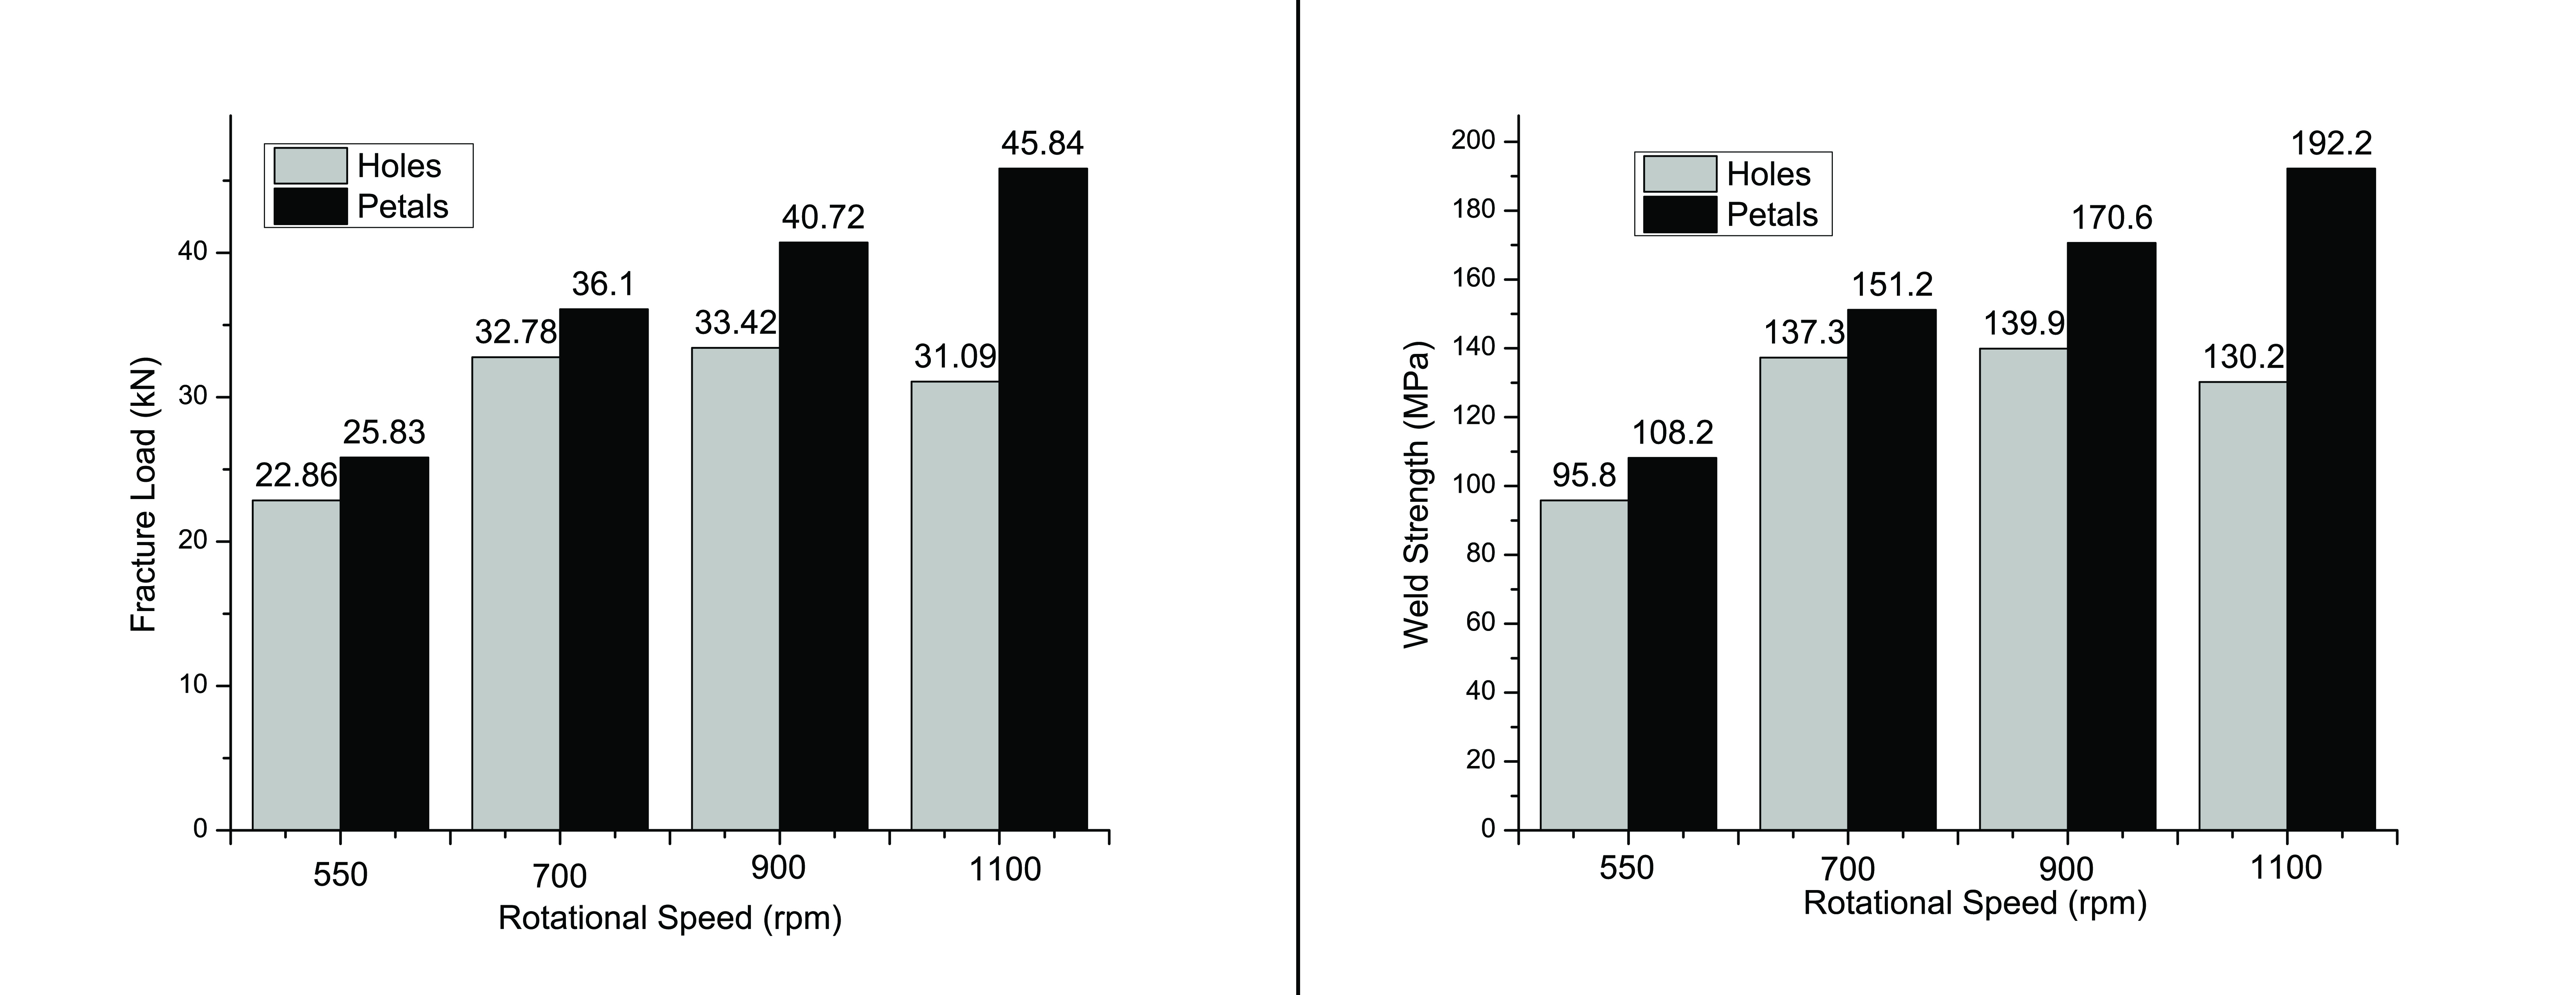
\includegraphics[width=\textwidth,keepaspectratio]{images/Strength.jpg}
\caption{Fracture load and Weld Strength of FWTPET welds}
\label{fig:weld-strength}
\end{figure}

\begin{figure}[!htbp]
\centering
\includegraphics[width=\textwidth,keepaspectratio]{images/MicroStructure.png}
\caption{XRD - Plot}
\label{fig:xrd-plot}
\end{figure}

\begin{figure}[!htbp]
\centering
\includegraphics[width=\textwidth,keepaspectratio]{images/MacroStructure.png}
\caption{XRD - Plot}
\label{fig:xrd-plot}
\end{figure}

\fi



%%%%%%%%%%%%%%%%%%%%%%%%%%%%%%%%%%%%%%%%%%%%%%%%%%%%%%%%%%%%%%%%%%%%%%%%%%
							%%References
%% Following citation commands can be used in the body text:
%% Usage of \cite is as follows:
%%   \cite{key}         ==>>  [#]
%%   \cite[chap. 2]{key} ==>> [#, chap. 2]
%%

%%%%%%%%%%%%%%%%%%%%%%%%%%%%%%%%%%
%% Elsevier bibliography styles %%
%%%%%%%%%%%%%%%%%%%%%%%%%%%%%%%%%%
%% Numbered
%\bibliographystyle{model1-num-names}

%% Numbered without titles
%\bibliographystyle{model1a-num-names}

%% Harvard
%\bibliographystyle{model2-names.bst}\biboptions{authoryear}

%% Vancouver numbered
%\usepackage{numcompress}\bibliographystyle{model3-num-names}

%% Vancouver name/year
%\usepackage{numcompress}\bibliographystyle{model4-names}\biboptions{authoryear}

%% APA style
%\bibliographystyle{model5-names}\biboptions{authoryear}

%% AMA style
%\usepackage{numcompress}\bibliographystyle{model6-num-names}

%% `Elsevier LaTeX' style
\bibliographystyle{elsarticle-num}

%% References with BibTeX database:
%% Authors are advised to use a BibTeX database file for their reference list.
%% The provided style file elsarticle-num.bst formats references in the required style

\bibliography{bibtex-database}

%% For references without a BibTeX database:

% \begin{thebibliography}{00}

%% \bibitem must have the following form:
%%   \bibitem{key}...
%%

% \bibitem{}

% \end{thebibliography}
%%%%%%%%%%%%%%%%%%%%%%%%%%%%%%%%%%%%%%%%%%%%%%%%%%%%%%%%%%%%%%%%%%%%%%%%%%
							%%Appendix
%% The Appendices part is started with the command \appendix;
%% appendix sections are then done as normal sections
%% \appendix

\end{document}